\documentclass{beamer}
\usepackage{graphicx}
\usepackage[utf8]{inputenc}
\usepackage{biblatex}
\usepackage{marvosym}
\setbeamercovered{transparent=15}
\addbibresource{../bibliography.bib}

\setbeamerfont{institute}{size=\large}
\setbeamerfont{date}{size=\small}

\newcommand\red[1]{\textcolor{red}{#1}}

\usetheme{Madrid}
\usecolortheme{orchid}

\title{Blockchain and Bitcoin}
\subtitle[]{Overview of Blockchain technology and cryptocurrencies, focusing on
the Bitcoin protocol and its scalability and privacy aspects}
\institute[]{Università degli studi di Brescia}
\author{Michele Zanotti}
\date{\today}

\begin{document}
  \begin{frame}
    \titlepage
  \end{frame}
  \begin{frame}{Summary}
    \tableofcontents
  \end{frame}

  %%%%%%%%%%%%%%%%%%%%%
  %%% FIRST SECTION %%%
  %%%%%%%%%%%%%%%%%%%%%
  \section{Introduction}
  \begin{frame}{Introduction}
    \framesubtitle{Distributed systems}
    \begin{columns}[onlytextwidth]
      \column{.5\textwidth} \begin{block}{Distributed system}
        A \textcolor{red}{distributed system} is a network that consists of autonomous nodes,
        connected using a distribution middleware, which acts in a coordinated way
        (passing messages to each other) in order to achieve a common outcome and
        that can be seen by the user as a single logical platform.
      \end{block}

      \column{.5\textwidth}
      \begin{figure}[!htb]
        \centering
        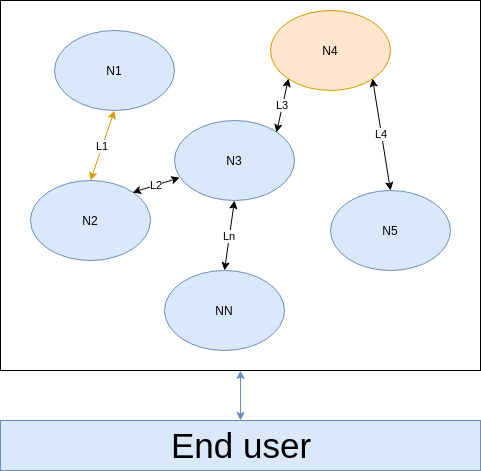
\includegraphics[width=0.7\linewidth]{../img/distributed-system.png}
      \end{figure}
    \end{columns}
  \end{frame}




  \begin{frame}{Introduction}
    \framesubtitle{Distributed systems}
      The desired properties of a distributed system are the following:\vspace{10pt}
      \begin{itemize}
        \item \textbf{Consistency}: all the nodes have the same lates available copy of the data.
        \item \textbf{Availability}: the system is always working and responding to the
        input requests without any failures.
        \item \textbf{Partition tolerance}: if a group of nodes fails the distributed system
        still continues to operate correctly
      \end{itemize}
  \end{frame}




  \begin{frame}{Introduction}
    \framesubtitle{Distributed systems}
    Even if some of the nodes fault or links break, a distributed system should tolerate
    this and should continue to work correctly. There are two types of fault:
    \begin{itemize}
      \item Simple node crash
      \item Exhibition of malicious or inconsistent behavior arbitrarily: \red{Byzantine fault}
    \end{itemize}

    \begin{block}{Byzantine nodes}
      A \textcolor{red}{Byzantine node} is a node that has an arbitrary behavior,
      which can even be malicious.
    \end{block}
  \end{frame}




  \begin{frame}{Introduction}
    \framesubtitle{Distributed systems}
    \begin{block}{Consensus}
      \red{Consensus} is the process of agreement between untrusted nodes on a data
      value.
    \end{block}

    Consensus mechanism requirements:
    \begin{itemize}
      \item \textbf{Agreement}: non-byzantine nodes must agree on the same value
      \item \textbf{Termination}: the consensus process must come to an end (nodes
      have to reach a decision)
      \item \textbf{Validity}: the agreed value must have been proposed by at
      least one honest node
      \item \textbf{Fault tolerance}: the consensus algorithm must work even
      in the presence of one or more Byzantine nodes
    \end{itemize}
  \end{frame}



  \begin{frame}{Introduction}
    \framesubtitle{Distributed systems}
    \begin{block}{The Byzantine generals problem}
      \begin{itemize}
        \item Problem formulated by Leslie Lamport \cite{lamport1982byzantine}
        \item A group of generals are surrounding a city and they have to agree
        on a common decision: attack or retreat.
        \item Their only communication way is a messenger
        \item Some of the generals may be \emph{traitors}: they communicate
        misleading message for preventing the loyal generals from reaching an
        agreement
        \item Requirement: algorithm that allows the loyal generals to agree
        on the same plan regardless of traitors general
      \end{itemize}
    \end{block}
  \end{frame}







  %%%%%%%%%%%%%%%%%%%%%
  %%% SECOND SECTION %%%
  %%%%%%%%%%%%%%%%%%%%%
  \section{Introduction to Blockchain}
  \subsection{Definition}

  \begin{frame}{What is Blockchain}
    \begin{block}{Business definition}
      Blockchain is a platform whereby peers can exchange values without the need
      for a central trusted party by using transactions which are stored inside
      the platform in a verifiable and permanent way.
    \end{block}

    \begin{block}{Technical definition}
      Blockchain is a distributed ledger that is
      \begin{itemize}
        \item cryptographically secure
        \item append-only
        \item immutable (extremely hard to change)
        \item updateable only via consensus among nodes
      \end{itemize}
    \end{block}
  \end{frame}



  \subsection{Features}
  \begin{frame}{Blockchain features}
    \begin{itemize}
      \item \textbf{Decentralization}: no need of a central trusted entity
      which stores the data and validates the transaction \pause
      \item \textbf{Distributed consensus}: high Byzantine Fault
      Tolerance, for each data value there's only a single version agreed by all
      parties through a consensus algorithm \pause
      \item \textbf{High availability}: Blockchain is based on a peer-to-peer
      network and data replicated on each node: even if one or more nodes fail
      the whole network can continue to work correctly
    \end{itemize}
  \end{frame}

  \begin{frame}{Blockchain features (Cont.)}
    \begin{itemize}
      \item \textbf{Immutability}: once a block has been added to the blockchain,
      changing it is computationally infeasible \pause
      \item \textbf{Transparency}: every node can see what is in the blockchain \pause
      \item \textbf{Security}: integrity of data, authentication and non-repudiation
      are ensured. Confidentiality is not provided. Security is a consequence of
      the distributed nature of Blockchain \pause
      \item \textbf{Uniqueness}: every transaction is unique and has not been spent already
    \end{itemize}
  \end{frame}



  \subsection{Structure}
  \begin{frame}{Blockchain structure}
    \begin{itemize}
      \item Linked list of ordered fixed-length \red{blocks}
      \item Each block includes a set of \red{transactions}
    \end{itemize}

    \begin{figure}[!htb]
      \centering
      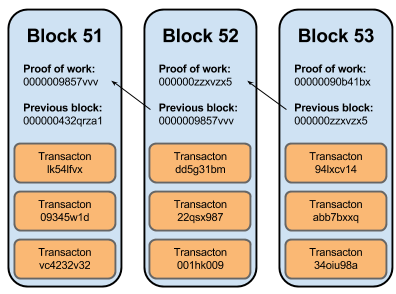
\includegraphics[width=0.45\linewidth]{../img/blockchain-basic-schema.png}
    \end{figure}
  \end{frame}




  \begin{frame}{Blockchain structure}
    \framesubtitle{Blocks structure}
      \begin{itemize}
        \item  A block is a group of transactions. Generally, it is composed of:
        \begin{itemize}
          \item[-] a set of transactions
          \item[-] a hash which identifies the block
          \item[-] a pointer to the previous block hash
          \item[-] a nonce
          \item[-] a timestamp
        \end{itemize}
        \item The first block in the blockchain is called \red{genesis block}.
      \end{itemize}
  \end{frame}




  \begin{frame}{Blockchain structure}
    \framesubtitle{Nodes, addresses and transactions}
    \begin{itemize}
      \item \textbf{Nodes} are active entities which store a copy of the blockchain and can
      perform and/or validate transactions \pause
      \item \textbf{Addresses} are unique identifiers which identify the parties involved in a
      transaction and usually are a public key or are derived from a public key. \pause
      \item \textbf{Transactions} are transfers of value from an address to another. \pause
      \item \textbf{Transaction scripts} are predefined sets of commands for nodes to transfer
      values from one address to another and perform various other functions.
    \end{itemize}
  \end{frame}



  \subsection{Consensus}
  \begin{frame}{Consensus in Blockchain}
    \begin{block}{Consensus}
      \begin{itemize}
        \item Required to establish whether the ledger itself or new blocks are
        valid or not
        \item Analogy with the Byzantine Generals Problem: ``generals'' are the nodes
        of the blockchain, ``messengers'' are the network links and ``traitors''
        are malicious nodes which try to tamper with the data
      \end{itemize}
    \end{block}
    \pause

    \begin{block}{Consensus mechanisms commonly used in Blockchain}
      \begin{itemize}
        \item Practical Byzantine Fault Tolerance (\textbf{PBFT})
        \item Proof of Work (\textbf{PoW})
        \item Proof of Stake (\textbf{PoS})
        \item Delegated Proof of Stake (\textbf{DPoS})
      \end{itemize}
    \end{block}
  \end{frame}




  \begin{frame}{Consensus in Blockchain}
    \begin{block}{Practical Byzantine Fault Tolerance}
      \begin{itemize}
        \item Algorithm proposed by M. Castro and B. Liskov as an optimized
        solution to the Byzantine Generals Problem \cite{castro1999practical} \pause
        \item Each “general” maintains an internal state. When he receives a
        message, he uses it in conjunction with his internal state to
        run a computation which tells what to think about the message in question \pause
        \item  After reaching his individual decision about the message,
        the general shares that decision with all the other “generals” in the system \pause
        \item  A consensus decision is determined based on the total decisions
        submitted by all generals \pause
        \item \textcolor{green}{Pro}: very efficient \pause
        \item \red{Cons}: precludes users anonimity \pause
        \item Mechanism adopted by Hyperledger and Ripple
      \end{itemize}
    \end{block}
  \end{frame}




  \begin{frame}{Consensus in Blockchain}
    \begin{block}{Proof of Work}
      \begin{itemize}
        \item Contrary to the PBFT, it doesn’t require all nodes to submit
        their individual conclusions \pause
        \item Based on a proof that ensures that enough computational resources have
        been spent before proposing a block for acceptance by the network \pause
        \item Only a single node (the first one who solves the PoW) announces its
        block \pause
        \item The announced blocks can be independently verified by all
        the nodes in the system \pause
        \item Mechanism adopted by Bitcoin
      \end{itemize}
    \end{block}
  \end{frame}





  \begin{frame}{Consensus in Blockchain}
    \begin{block}{Proof of Stake}
      \begin{itemize}
        \item Contrary to PoW, there isn't any individual attempting to carry out
        an intensive computation in order to propose a block \pause
        \item The network runs a lottery based on the nodes’ stake to decide
        who will announce a block \pause
        \item The more stake one node has, the higher the probability
        to be chosen is \pause
        \item Main idea: if a node that has enough stake in the system it means
        that it has invested enough in the system \MVRightarrow\, any malicious
        attempt/attack on the system wouldn't have any benefits for him \pause
        \item \red{Main problem}: the system rewards more those who already are most
        deeply involved in the network \MVRightarrow\, the system becomes always
        more centralized
      \end{itemize}
    \end{block}
  \end{frame}





  \begin{frame}{Consensus in Blockchain}
    \begin{block}{Delegated Proof of Stake}
      \begin{itemize}
        \item Evolution of the PoS \pause
        \item Each node that has stake in the system can choose an entity to
        represent its portion of stake in the system (by voting) \pause
        \item The more stake one node has, the higher is the weight of his vote \pause
        \item The entity with most votes (weighted) becomes a delegate which
        proposes blocks \pause
        \item The voting process is periodically executed: if the current delegate
        doesn't behave correctly the other nodes just stop voting it
      \end{itemize}
    \end{block}
  \end{frame}



  \subsection{Types of Blockchain}
  \begin{frame}{Types of Blockchain}
    \begin{block}{Public Blockchain}
      \begin{itemize}
        \item Blockchain open to the public in which everyone can join the network,
        maintain the shared ledger and participate in the consensus process \pause
        \item The ledger is not owned by anyone and everyone can read it \pause
        \item Usually there's an incentive mechanism to encourage more participants
        to join the network \pause
        \item \red{Main problem}: lack of privacy (everyone can see the transactions
        stored in the blockchain) \pause
        \item Bitcoin is based on a public blockchain
      \end{itemize}
    \end{block}
  \end{frame}




  \begin{frame}{Types of Blockchain (Cont. 1)}
    \begin{block}{Private Blockchain}
      \begin{itemize}
        \item Open only to an organization or a group of individuals \pause
        \item Participants need to obtain an invitation or permission to
        join the Blockchain and maintain the ledger \pause
        \item Usually the network is permissioned: restrictions on who is
        allowed to participate in the network and only in certain transactions
      \end{itemize}
    \end{block}
  \end{frame}




  \begin{frame}{Types of Blockchain (Cont. 2)}
    \begin{block}{Consortium Blockchain}
      \begin{itemize}
        \item Consensus process is controlled by a preselected set of nodes
        (e.g. a consortium of organizations, each of which operates a node) \pause
        \item  The right to read the blockchain might be public or permissioned
      \end{itemize}
    \end{block}
  \end{frame}










  %%%%%%%%%%%%%%%%%%%%%
  %%% THIRD SECTION %%%
  %%%%%%%%%%%%%%%%%%%%%
  \section{Bitcoin}
  \begin{frame}{}

  \end{frame}













  \begin{frame}{References}
    \printbibliography
  \end{frame}

\end{document}
